\documentclass[12pt,a4paper,]{article}
\usepackage[latin1]{inputenc}
\usepackage{amsmath}
\usepackage{amsfonts}
\usepackage{amssymb}
\usepackage{graphicx}
\author{haidai HU}

\title{Structural study of bacterial pentameric liganded gated ion channels}
\begin{document}
	\maketitle
	Pentameric liganded gated ion channels (PentaLGICs) are vital for nerve cells communication in central and peripheral nervous systems  in  animal kingdoms. The very first member of this family been characterised and isolated is nicotine receptor \cite{changeux1970use}. Receptors from this family can be divided into two sub\_families according to the permeated ions property. Cationic channel, such as Serotonin gated ion channels (5-HT$_3$R) and  nicotine Acetylcholine gated ion channels (nAChRs); Anionic channel, such as  $\gamma$ -amminobutyric acid gated ion channels(GABARs) and glycine gated ion channels (GlyRs). Binding of neurotransmitters  to the extra-cellar domain (ECD) of the receptor will trigger the trans-membrane domain (TMD) from closed to open and let the ions permeate through. This rapid progress facilitate the intercellular signalling.  Dysfunction of these receptors causes many diseases, such as 
	pain, Parkinson's Disease (PD), Alzheimer's Disease (AD), and other central nervous disorder diseases. Also receptors from these family involved in nicotine addition, drug addition. Numerous studies revealed that therapeutic compounds including propofol, desflurane, benzodiazepine, barbiturates, can target to PentaLGICs.\\ 
	%caffeine, alcohol \\
	%\begin{figure}
		%\caption{A picture of a gull.}
		%\centering
		%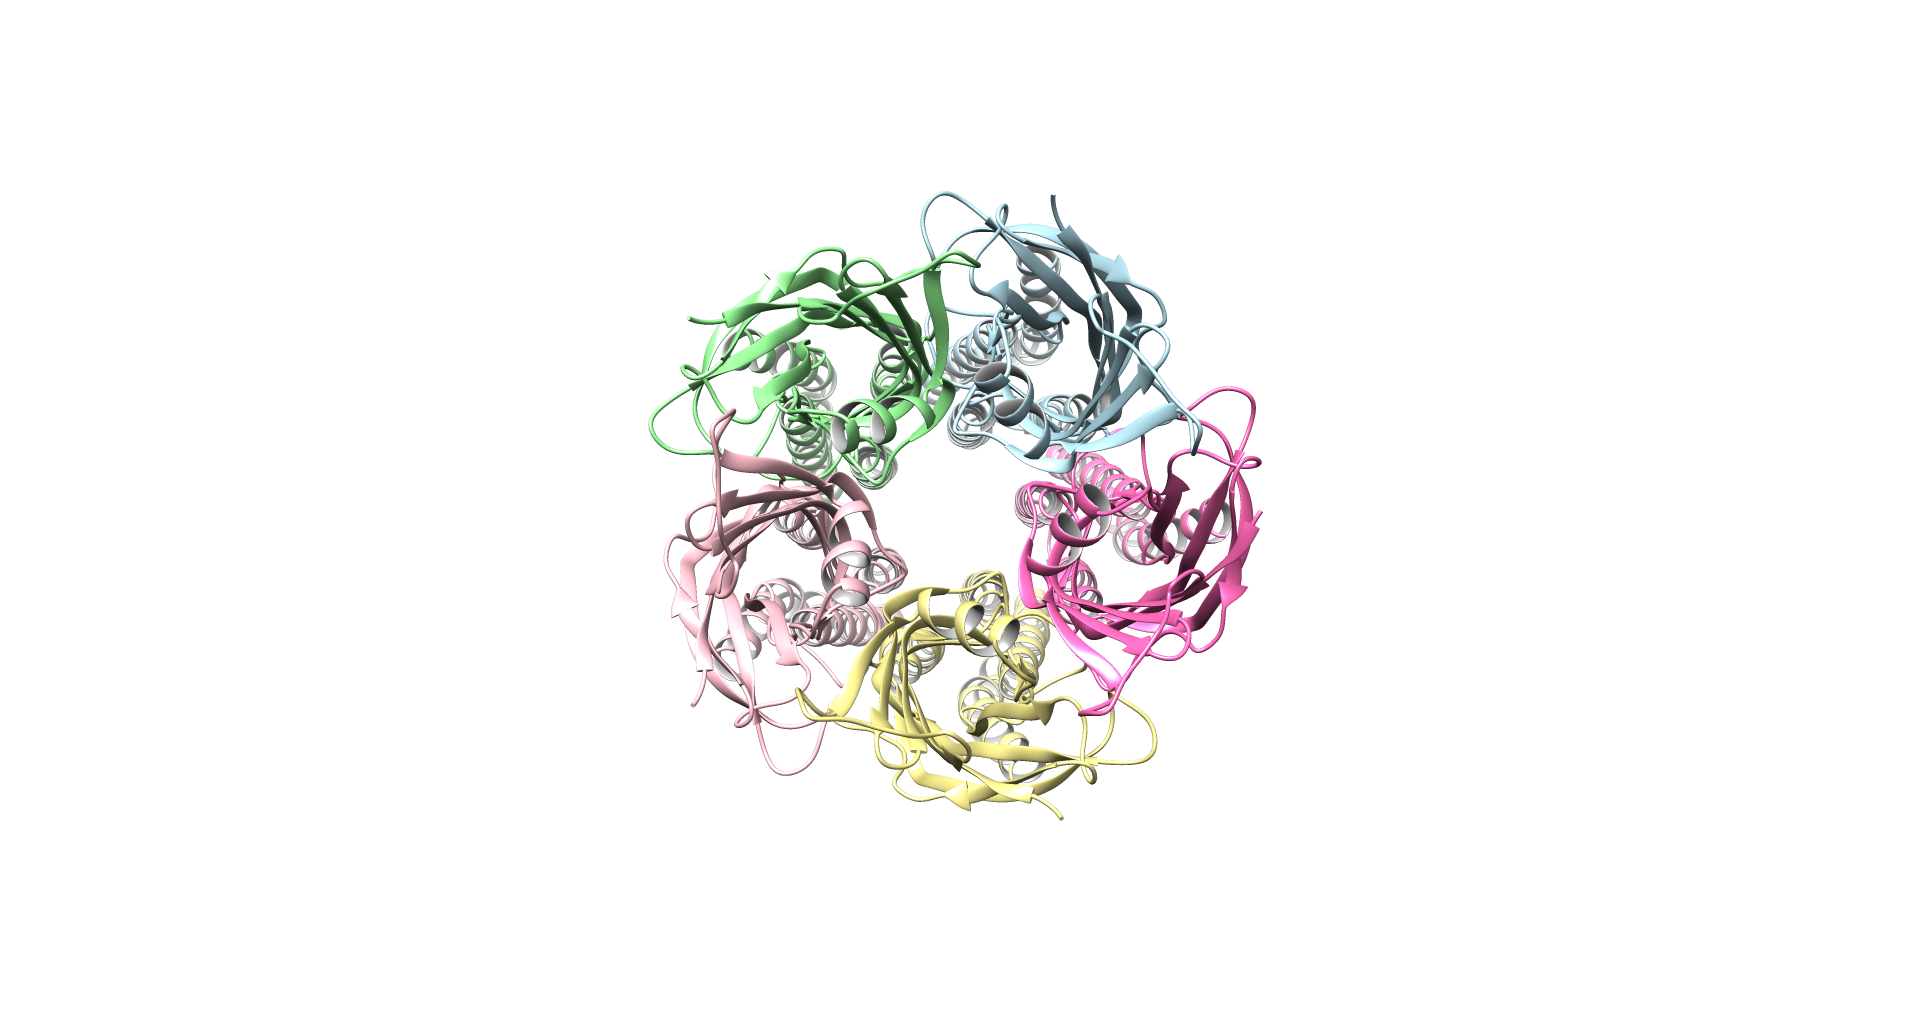
\includegraphics[width=0.5\textwidth, ]{figure_sTeLIC/figure1b}
	%\end{figure}
	
	
	
	
	
	
	
	
	In eukaryote, duo to the highly conserved characteristic disulfide bond, which is formed by two Cysteines aparted by 13 conserved amino acids, locating at the interface of  ECD and TMD,  pentaLGIC are also called cys-loop receptors. Year of 2005, based on sensitive sequence-profile searches, using ECD of known cys-loop receptors as seeds,  \textsl{Asba tasneem et al.}, identified several putative homologs of cys-loop receptors from prokaryote.
	One of them ,which is  from $\textsl{Gleobacter violaceus}$, a genus of cyanobacteria, was subsequently demonstrate as a cationic proton-gated ion channel and can be over-expressed using $\textsl{E.coli}$ expression system with the N terminal of receptor fused with Maltose binding protein \cite{boc07}.This receptor,  termed as GLIC, provide the first apparently atomic open form conformation of PentaLGICs\cite{hilf2009structure}. Together with the closed form of ELIC ($\textsl{Erwinia chrysanthemi}$ ligand-gated ion channel) which structure was determined also using X-ray crystallography at 3.3 \AA{} \cite{hilf2008x} resolution, pave the way for us to understand the mechanism of "gating". Later, the first crystal structure of invertebrate anion-selective cys-loop receptor from \textsl{Caenorhabditis elegans} was solved with the help of  crystallization chaperone Feb. Following, atomic details of several eukaryote pentalGIC receptors were characterised either using crystallography or cryo-microscopy. These invaluable structural information extend our konwledge about PentaLGICs. \\ 
	
	GLIC, a proton gated cationic channel, which structural conformation is sensitive to environment pH, has been studied for about ten years. First, GLIC structure was solve at pH 4 with the ion channel pore diameter  larger enough for cationic ions $Na^+$ and $K^+$ pass through. Second, by ether cross linking between the \textsl{loop} 2 and M2-M3  \textsl{loop} or single mutant key amino acid located at M2 helix, \textsl{Prevost et al}  captured the receptor at "\textsl{Locally closed}" or  so called LC form. The ECD of LC  show the same configuration as the open form of GLIC, However, the TMD of LC form undergo a striking conformational change, with the upper part of M2 helix detach from inner subunit M3 helix bend and interact with the M2 helix form neighbour subunit. Consequence of structural rearrangement of this region cause the ion channel pore shrink and too small to let the ions permeate through. Third, after extensively screen crystals which grow form pH 7 environment, \textsl{Ludovic et al} successfully solve the resting state structure of GLIC. Even with moderate resolution (4.35\AA{}),  clearly quaternary change can be observed at the ECD and TMD comparing  with the open form of GLIC. On one hand , ECD of resting form undergo twist and blooming motion, on the other hand, TMD of resting form adopts the same pore conformation as found from LC form.\newpage
	
	
	
{\large 1. Poential proton binding sites of GLIC}\\	
	
Agonist of GLCI  is proton, which size  is too small to visualised through X-ray crystallography. 
We systematically mutant the negative charged  aspartic acid, glutamic acid ( $pK_a$ value of carboxyl group is 3.71 and 4.15 respectively)  as well as Histidine ($pK_a$ value of imidazole is 6.04). 
%The sites we chose to mutant are either located at the ECD interface of intra subunit which will be  protonated at acidic pH and deprotonated at n
	\begin{figure}
	\caption{Phenotype of GLIC potential proton binding sites mutants}
	\centering
	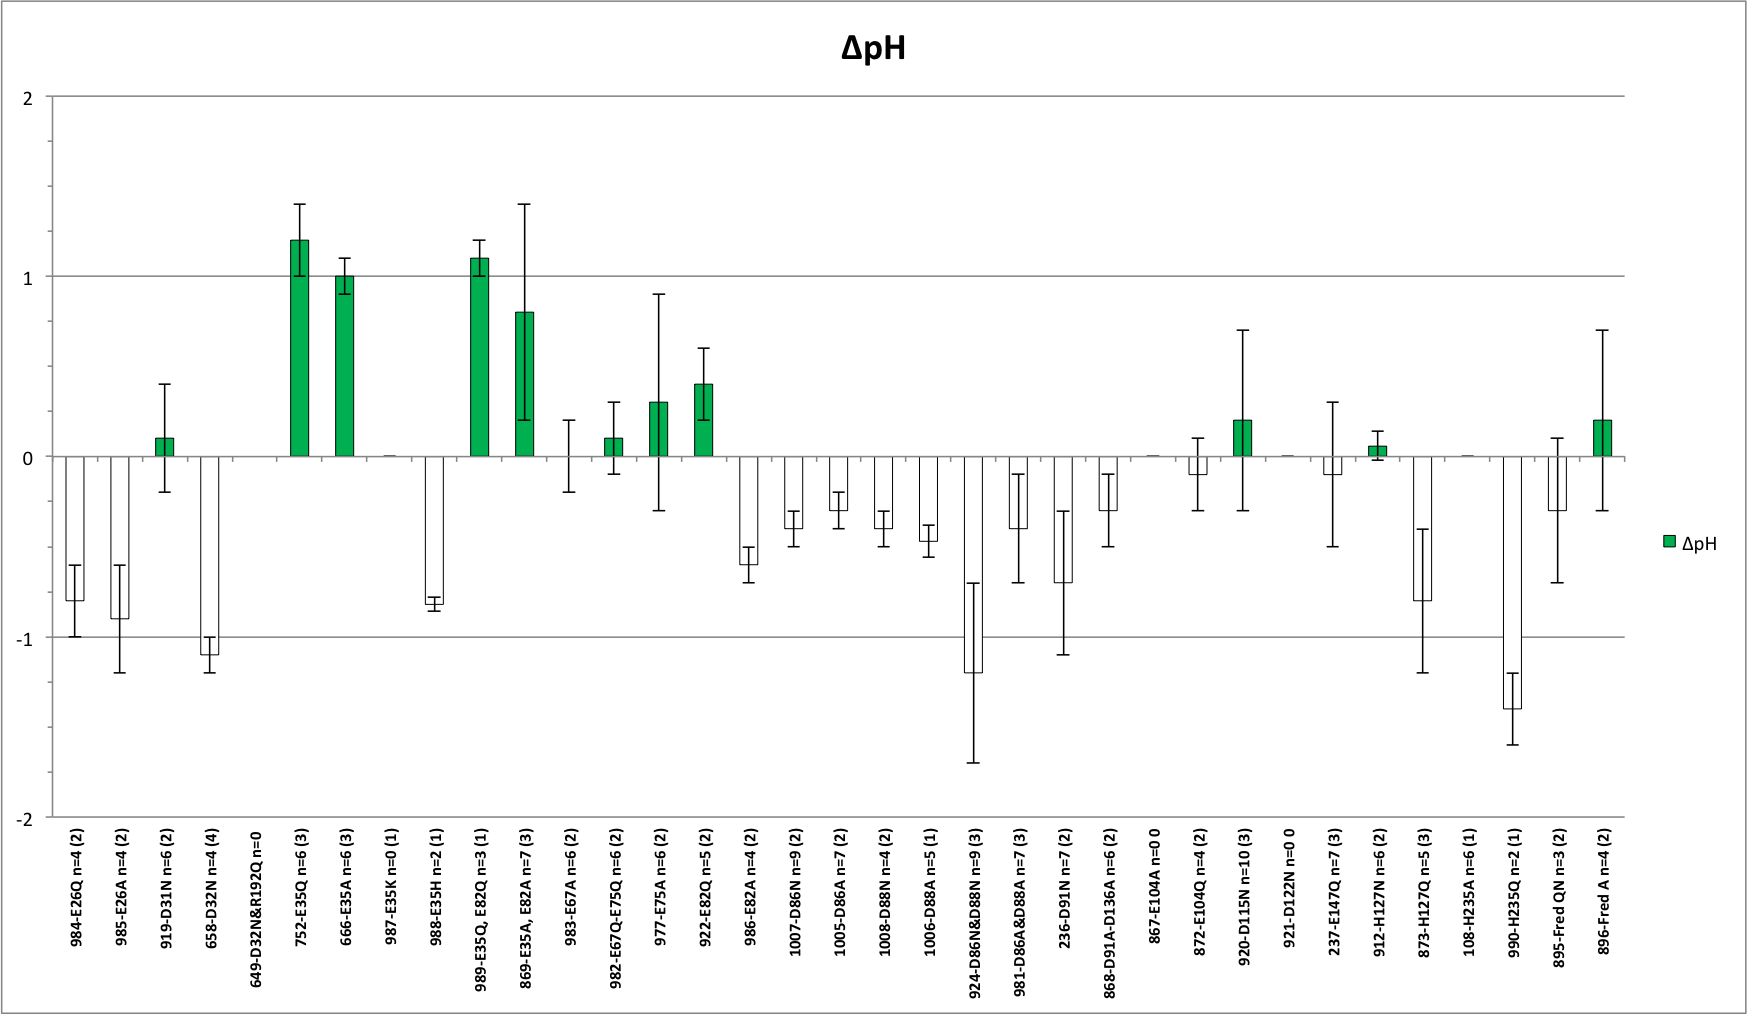
\includegraphics[width=1\textwidth, ]{figure_GLIC/functional_result}
	\end{figure}\\
	
Preliminary conclusion:\\
	(1) Proton binding site is not single spot, since single mutation will not cause GLIC insensitive to proton.\\
	(2) Double or triple mutation will accumulate the "loss of  function" phenotype implying the exist of  putative proton binding network.\\
	(3) Mutation potential proton binding site of E35 shows "gain of function" suggesting that this special sites may play other  unknown roles.\\
	
	{\large 2. Pre\_M1 region of GLIC participate in channel gating }\\
	
 During the process that we try to identify proton binding sites of GLIC, we notice that one  of amino acid E35, which is located at the tip of $\beta$1-$\beta$2 {\textsl loop} facing neighbour subunit {\textsl loop}F and pre\_M1 region, mutation of  E35A and E35Q have strong "gain of function"phenotype. 
 %When mutate E35 to polor unchanged glutamine, it shows "gain of function " phenotype. When mutate E35 to alanine, "gain of function" increase. when convert negative charged glutamate to positive charged  histidine, the receptor shows "loss of function". 
 In the high resolution structure of GLIC wt, in the region E35, pre\_M1* and \textsl{loop} F* (*represent residues from adjacent subunit ), we find three water molecules. Through these water molecules, by forming hydrogen bonds, Q193* connects E35, M2\_M3 loop,  and \textsl{loop} F*. We show that replacement of glutamine to hydrophobic amino acid leucine or  methionine causes the ion channel pore from open to close. In agreement with structural conformation change, functional experiment shows "loss of function" phenotype of Q193M and Q193L. Further, we shorten the side chain  of glutamine 193 by replacing it with cysteine. It shows Q193C has the same functional phenotype as WT GLIC. Structural analysis shows that the introduced cysteine form new type of hydrogen bonds that maintain ion channel pore open. Additional, blocking the cysteine with S-Methyl methanethiosulfonate(MTS) cause the ion channel close again. Our experiments show the important role of Q193 that participate in ion channel gating. Since this residue is also conserved in other human PentalGIC like glycine receptor, the mechanism here may apply within the family. \\
 
 
 {\large 3. Crystal structure of a PentaLGIC }\\	
 
Year of 2005, based on sensitive sequence-profile searches, using ECD of known cys-loop receptors as seeds,  \textsl{Asba tasneem et al.}, identified several putative homologs of cys-loop receptors from prokaryote.
One of them ,which is  from $\textsl{Gleobacter violaceus}$, a genus of cyanobacteria, was subsequently demonstrate as a cationic proton-gated ion channel and can be over-expressed using $\textsl{E.coli}$ expression system with the N terminal of receptor fused with Maltose binding protein \cite{boc07}.This receptor,  termed as GLIC, provide the first apparently atomic open form conformation of PentaLGICs\cite{hilf2009structure}. Together with the closed form of ELIC ($\textsl{Erwinia chrysanthemi}$ ligand-gated ion channel) which structure was determined also using X-ray crystallography at 3.3 \AA{} \cite{hilf2008x} resolution, pave the way for us to understand the mechanism of "gating". Later, the first crystal structure of invertebrate anion-selective cys-loop receptor from \textsl{Caenorhabditis elegans} was solved with the help of  crystallization chaperone Feb. Following, atomic details of several eukaryote pentalGIC receptors were characterised either using crystallography or cryo-microscopy. These invaluable structural information extend our konwledge about PentaLGICs. Here, We determine crystal structure of another PentaLGIC form symbiont of Tevnia (sTeLIC) at 2.5 \AA{} resolution. Structural analysis shows two positive charged filters constrain the ion pass way at the extra-cellar domain, while, largest ion channel pore form by M2 helix provide no restriction for ion permeation in the trans-membrane domain. The newly structural architecture  presented here extend our view about "gate" in the family of PentalGIC.
 
 
	
	
	   %%he X-ray structure of the GluCl?Fab complex was determined with the allosteric agonist ivermectin and in additional structures with the endogenous neurotransmitter L-glutamate and the open-channel blocker picrotoxin. 
%%	In prokaryote receptors, even though the absence of  circled  cys-loop  formed  by cysteine pair,  the overall  structure construction are the same as the sturcture of nAChR which  was solved using Cryo-EM method at 4 \AA{} resolution. Another striking difference is that the exist of  cytoplasmic  domain in eukaryote receptors is missing in prokaryote receptors. Deleting the Cytoplasmic domain of 5-HT$_3$ and. So  receptors from prokaryote may represent the minimum  functional part of PentalGIC.



%%PentaLGICs belong to the transmembrane proteins, with five monomers  symmetrically arrange along the five-fold symmetry axis. For each monomer , N-termianl ECD folded into $\beta$ sandwich conformation followed by four transmembrane $\alpha$ helices (M1-M4). M1 helix connect to ECD directly and M4 helices face to the membrane environment. Five M2 helix contributed by five monomers border the ion channel pore.
	% The ion channel pore formed by five M2 helix contributed by five monomers 
	% Five M2 helix contributed by five monomers border the ion channel pore.      
	
	
	
	
	%Since the important role of the PentaLGIC, 
	
	
	%central and peripheral nervous systems
	%In animal kingdom, because of the conserved 
	%disulfate bonds formed by 
	
	\bibliographystyle{plain}
	\bibliography{myreference_PentalGLIC.bib}
\end{document}